% Fig 1: system overview (two panels).
% Compile standalone:  pdflatex fig1_system.tex  ->  include fig1_system.pdf
% Requires: \usepackage{tikz} is NOT needed in main doc if included as PDF.
% NOTE: scale=0.76 shrinks geometry to ~3.5in (single column) while keeping
% node text at design size (\small=9pt, \footnotesize=8pt) — no font shrinkage.
\documentclass[tikz,border=4pt]{standalone}
\usetikzlibrary{arrows.meta,positioning,calc}
\begin{document}
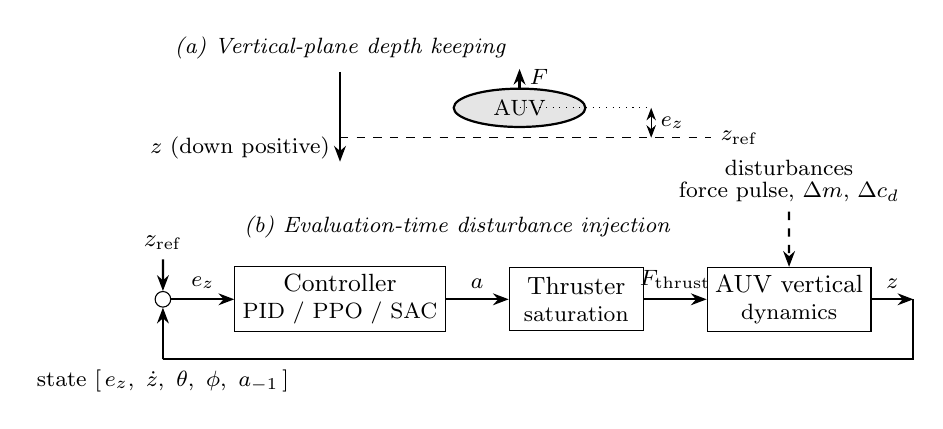
\begin{tikzpicture}[
  scale=0.76,
  font=\small,
  blk/.style={draw, minimum height=8mm, minimum width=17mm, align=center, inner sep=1mm},
  sumnode/.style={draw, circle, inner sep=0.7mm},
  arr/.style={-{Stealth[length=2mm]}, thick},
  lbl/.style={font=\footnotesize},
]

% ================= (a) vertical-plane coordinates =================
\begin{scope}[shift={(0,0)}]
  % z axis (down positive)
  \draw[arr] (0,0) -- (0,-15mm) node[left, lbl, pos=0.85]{$z$ (down positive)};
  % target depth line
  \draw[dashed] (0,-11mm) -- ++(62mm,0) node[right, lbl]{$z_{\mathrm{ref}}$};
  % AUV body
  \draw[fill=gray!20, thick] (30mm,-6mm) ellipse (11mm and 3.2mm);
  \node[lbl] at (30mm,-6mm) {AUV};
  % thruster arrow
  \draw[arr] (30mm,-2.8mm) -- (30mm,0.5mm) node[right, lbl, pos=0.6]{$F$};
  % depth error bracket
  \draw[dotted] (30mm,-6mm) -- (52mm,-6mm);
  \draw[{Stealth[length=1.6mm]}-{Stealth[length=1.6mm]}] (52mm,-6mm) -- (52mm,-11mm)
        node[midway, right, lbl]{$e_z$};
  \node[lbl, font=\footnotesize\itshape] at (0,4mm) {(a) Vertical-plane depth keeping};
\end{scope}

% ================= (b) control loop =================
\begin{scope}[shift={(0,-38mm)}]
  \node[blk] (ctrl) {Controller\\[-0.5mm]{\footnotesize PID / PPO / SAC}};
  \node[blk, right=8mm of ctrl] (thr) {Thruster\\[-0.5mm]{\footnotesize saturation}};
  \node[blk, right=8mm of thr] (dyn) {AUV vertical\\[-0.5mm]{\footnotesize dynamics}};
  \node[sumnode, left=8mm of ctrl] (sum) {};
  \node[above=4mm of sum] (ref) {$z_{\mathrm{ref}}$};

  \draw[arr] (ref) -- (sum);
  \draw[arr] (sum) -- node[lbl, above]{$e_z$} (ctrl);
  \draw[arr] (ctrl) -- node[lbl, above]{$a$} (thr);
  \draw[arr] (thr) -- node[lbl, above]{$F_{\mathrm{thrust}}$} (dyn);
  \draw[arr] (dyn.east) -- ++(7mm,0) coordinate (out) node[midway, above, lbl]{$z$};

  % feedback
  \draw[arr] (out) |- ($(sum)+(0,-10mm)$) -| (sum) node[pos=0.25, below, lbl]{state $[\,e_z,\ \dot z,\ \theta,\ \phi,\ a_{-1}\,]$};

  % disturbances entering dynamics
  \node[above=7mm of dyn, lbl, align=center] (dist) {disturbances\\[-0.5mm]{\footnotesize force pulse, $\Delta m$, $\Delta c_d$}};
  \draw[arr, dashed] (dist) -- (dyn);

  \node[lbl, font=\footnotesize\itshape, anchor=south west] at ($(ctrl.north west)+(0,3mm)$) {(b) Evaluation-time disturbance injection};
\end{scope}

\end{tikzpicture}
\end{document}
